\documentclass[a4paper,10pt]{article}
\usepackage[utf8]{inputenc}
\usepackage{graphicx}
\usepackage{subcaption}
\usepackage{parskip}
\usepackage{amsmath}
\usepackage{listings}
\usepackage{color}
\usepackage{listings}

\definecolor{red}{rgb}{1,0,0}
\definecolor{green}{rgb}{0,1,0}
\definecolor{codegreen}{rgb}{0,0.6,0}
\definecolor{codegray}{rgb}{0.5,0.5,0.5}
\definecolor{codepurple}{rgb}{0.58,0,0.82}
\definecolor{backcolour}{rgb}{0.95,0.95,0.92}

\lstdefinestyle{mystyle}{
    backgroundcolor=\color{backcolour},   
    commentstyle=\color{blue},
    numberstyle=\tiny\color{codepurple},
    stringstyle=\color{codegreen},
    basicstyle=\footnotesize,
    breakatwhitespace=false,         
    breaklines=true,                 
    captionpos=b,                    
    keepspaces=true,                 
    numbers=left,                    
    numbersep=5pt,                  
    showspaces=false,                
    showstringspaces=false,
    showtabs=false,                  
    tabsize=2
}
 
\lstset{style=mystyle,language = C}

%opening
\title{UNIK4690 Prosjektforslag\\ Virtual Reality}
\author{Joseph Knutson \& Jacob Hay}

\begin{document}

\maketitle
\section*{Prosjektbeskrivelse}
\begin{itemize}
%  \item Vi ønsker først og fremst å lage en 3D modell av scenen (et enkelt rom) ut ifra et ubestemt antall statisk oppstilte kameraer. %(bonus hvis vi får tid: Selv om kameraene er statiske vil vi skape et 3rd person view ( se fig \ref{fig1}).
\item Vi vil lage real-time avatarer av oss selv og projisere dem inn i en 3D scene. For å mappe kroppene våres vil vi utnytte OpenPose\footnote[1]{Kult library for real-time pose estimering av mennesker: https://github.com/CMU-Perceptual-Computing-Lab/openpose} biblioteket (se fig \ref{fig1}) som vil danne grunnlag for avatarenes skjellett.
\item For at avataren skal kunne interagere med en 3D scene vil vi gi den en såkalt "hitbox" som omhyller dens skjellett. Dette vil vi prøve å få til ved hjelp av openFrameworks (se figur \ref{fig2}).
\item Vi ønsker også å leke oss litt med scenen ved å legge til teksturer på både den og avataren, så får simuleringen en slags gaming/vrchat følelse.
\item Hvis det blir tid vil vi inkludere diverse objekter i scenen som avatarer kan interagere med ved hjelp av fysikkverktøy fra OpenFrameworks.
\end{itemize}
\clearpage

% 
% \begin{figure}\centering
%  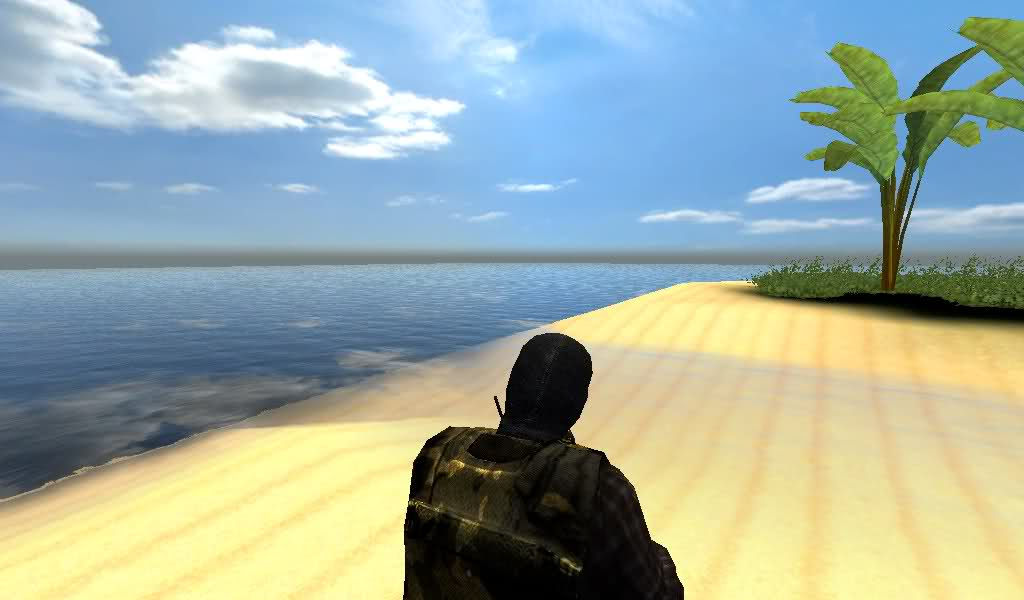
\includegraphics[width = 0.8\linewidth]{3rd}
%  \caption{Overblikket vi ønsker å skape.}
%  \label{fig1}
% \end{figure}


\begin{figure}\centering
 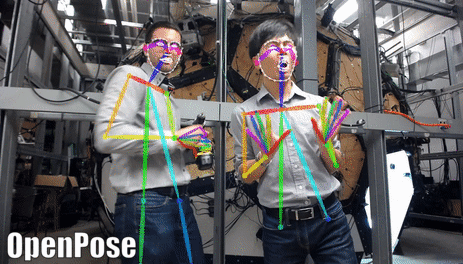
\includegraphics[width = 0.8\linewidth]{openpose}
 \caption{Med OpenPose will we "mappe" oss selv til en 3D scene.}
 \label{fig1}
\end{figure}

\begin{figure}\centering
 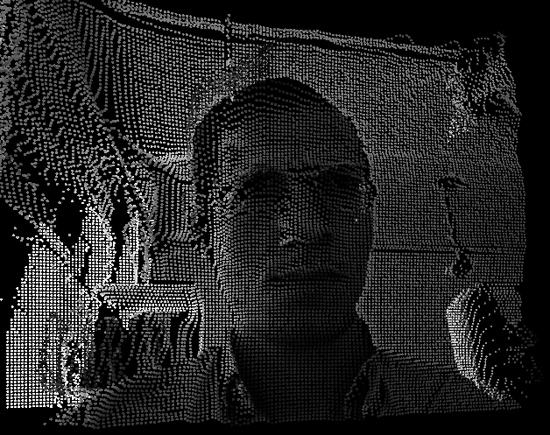
\includegraphics[width = 0.8\linewidth]{hitbox}
 \caption{En omhyllingskurve rundt en dude. Vi ønsker å bruke denne koden til å lage en enklere omhyllingskurve rundt avatarene.}
 \label{fig2}
\end{figure}

\end{document}
